\documentclass[11pt]{article}

%\usepackage{afterpage}

%\usepackage{pdflscape}
\usepackage{lscape}


\usepackage{geometry}
\geometry{a4paper,left=10mm, right=10mm, top=20mm, bottom=20mm}

\usepackage{graphicx}
\graphicspath{ {images/} }

\usepackage{tabularx}
\usepackage{colortbl}

\usepackage{fancyhdr}
\fancyhf{}
\lhead{Escort The President}
\rhead{System Requirements Specification}
\rfoot{Page \thepage}

\usepackage{enumitem}

\setcounter{tocdepth}{2}

\newcommand{\f}{\cellcolor{black}}

% You must use this in a subsubsection.
\newenvironment{req} {\begin{enumerate}[leftmargin=2.5cm, label = \textbf{REQ \arabic{subsection}.\arabic{subsubsection}.\arabic*:}]} {\end{enumerate}}


\begin{document}

\begin{flushright}
    \rule{16cm}{5pt}
    \vskip1cm
    \begin{bfseries}
        \Huge{Team Project}\\
        \vspace{1.9cm}
        \Huge{SOFTWARE REQUIREMENTS\\ SPECIFICATION}\\
        \vspace{1.9cm}
        for\\
        \vspace{1.9cm}
        Escort The President\\
        \vspace{1.9cm}
        Prepared by Team A1\\
        \vspace{1.9cm}
        James Birch, Ahmed Bhallo, Edward Dean, Brendan Hart, Kwong Hei Tsang\\
        \vspace{1.9cm}
        \today\\
    \end{bfseries}
    \vskip1cm
    \rule{16cm}{5pt}
\end{flushright}

\newpage

\pagestyle{fancy}
\tableofcontents

\newpage

\section{Introduction}
\subsection{Purpose}
We are team A1, designing and implementing the game "Escort The President". The purpose of this System Requirements document is to specify the overall system requirements that will govern the development and implementation of our game.

\subsection{Game Concept}
Escort The President is a multiplayer game where each rounds consists of Assassins attempting to assassinate the recently-elect president. Assassins carefully plot their move to kill the president, knowing there's a $\$ 2,000,000$ bounty awaiting. The president has been followed inside his car and he receives a tip that Assassins are patiently waiting to make their move... Gunshot! An Assassin has shot at the vehicle and the president's Escorts with the aid of Police Officers attempt to escort him to the helicopter \emph{alive}. To make matters worse, this is in public streets and there are civilians everywhere!

\subsection{Research}
\subsubsection{Target Audience}
Our target audience are teenagers from the age of 12 - 18 who enjoy fast-paced action shooter games. Because of this, our game must be engaging and aesthetically suited to meet our audiences' preferences.

\subsubsection{Perspective}
We have decided to go for a 2.5D top-down perspective, but not a direct birds-eye view in order to give depth to boundaries such as walls \cite{perspective}. This will grant players the freedom to move in 8 directions and feel in control of their unit. The game will only have 2 layers of depth (in order to not be confusing) -- The ground tiles (the floor), and the obstacle tiles (think of boxes and walls placed on the ground that are the size of a character).

\subsubsection{Character Movement}
When the creator of Super Mario Bros, Shigeru Miyamoto, was asked why the Mario franchise was so popular, he talked about the way they implemented movement \cite{miyamoto}. One element of Mario's movement was his slide (he doesn't stop moving exactly when a button is released). This is something we are planning to implement in our own game to make movement feel more natural, making our players feel immersed into the game.

\subsubsection{Sprites}
Unit rendering will require multiple different sprites depending on the direction they are facing. 1 base sprite for animation will be created, which will be used for every unit. In order to give units their uniqueness, sprites will programatically be modified on load (for example, changing the colour of clothes/skin, adding hair/hats).

\subsubsection{Sound and Music}
The game must have arcade-sounding sound effects and chip-tune music to give the game a nostalgic arcade feel.

\subsubsection{Networking}
Both TCP and UDP will be used as the transfer protocol on the server and client implementation in order to make the game work in most network environments. The player will be allowed to select which protocol to use during log on.

\paragraph{TCP} TCP provides a mechanism to guarantee any messages sent between server and the client reaching each other. Libraries for encryption are also ready for use to secure the data sent between the server and client. It is useful if the client is connecting through an insecure network such as public WiFi or a restrictive network which prevents UDP from working properly.

\paragraph{UDP} UDP does not guarantee each packet can reach each side as packet loss are not handled by the protocol. The benefit from it is not all lost messages have to be resent as they may be out of date such as the game state. This allows server and client to selectively resend important lost information only, increasing efficiency. At the same time, it reduces handshaking to reduce the delay. It is useful if the player is far away from the server or is connecting through a trusted network.\\

\noindent
Other parts of the game will only use MessageControl interface to send or receive objects of the Message class to avoid interacting directly with the networking subsystem. If the client and server is communicating via UDP, the networking module will determine whether specific message is critical or not to decide whether to resend the message when the other side fails to receive it.


\subsection{Glossary and Acronyms}
\begin{itemize}
	\item HP: Health Points
	\item Ammo: Weapon ammunition
	\item Mags: Ammunition magazines
	\item Combat activity: Combat activity occurs when a unit attempts to attack (by shooting for throwing a grenade).
	\item HUD: Head-up display. Visually relaying information as part of the user interface.
\end{itemize}

\subsection{References}
\begingroup \renewcommand{\section}[2]{} \begin{thebibliography}{}

\bibitem{perspective}
Brandon Dollar: Types of Game Perspectives,
\\\texttt{https://mozzastryl.wordpress.com/2013/01/20/types-of-game-perspectives/}

\bibitem{miyamoto} 
Shigeru Miyamoto: Miyamoto on World 1-1: How Nintendo made Mario's most iconic level,
\\\texttt{https://www.youtube.com/watch?v=zRGRJRUWafY}

\end{thebibliography} \endgroup

\section{System Features}
We have documented the features of our game in the form of functional requirements.

\subsection{Units}
A unit is a "character" of our game. Units in our game are the President, Escorts, Assassins (including Menaces), and Police Officers.

\subsubsection{Unit assignment}
\begin{req}
	\item The lobby system must randomly assign all human players a role of either Escort or Assassin at the beginning of each round.
	\item The lobby system must ensure that a ratio of 1 Escort for every 2 Assassins is maintained. If there are not enough human players to form assassins, the numbers must be made up with AI players.
	\item The lobby system must assign around 20 AI players to civilians.
\end{req}

\subsubsection{President (AI only)}
\begin{req}
	\item The president AI must remain stationary in his position until an Escort asks to follow. This is done by an Escort by walking up near to the president and pressing the Action key.
	\item When following an Escort, the president must find the path from the president's current position to the Escort's current position. The path must be recomputed every time the Escort makes a new move.
	\item Damage dealt by Escorts have no effect on the president.
\end{req}

\subsubsection{Escort (Human only)}
It is the Escorts' duty to ensure the safety of the president. They must fend off and kill Assassins while escorting the president to the save zone.
\begin{req}
	\item Damage dealt by Escorts have no effect on other Escorts.
	\item All Escorts win when the president has safely reached the safe zone.
\end{req}

\subsubsection{Assassins (Human and AI)}
The Assassins' goal is to be the one to kill the president. Only the assassin who dealt the killing blow to the president will win the game.
\begin{req}
    \item When an Assassin deals the killing blow to a civilian, they become a menace for 20 seconds.
	\item Damage dealt by Assassins have no effect on other Assassins.
	\item Damage dealt by Menaces \emph{do} have an effect on Assassins.
\end{req}

\subsubsection{Menace (Human and AI)}
A Menace is an Assassin who has recently killed a civilian. Menaces return back to normal Assassins after a set period of time (20 seconds). It is beneficial for Assassins to kill a Menace to relieve the competition of being the one to kill the president.
\begin{req}
	\item Damage dealt by Assassins \emph{do} have an effect on Menaces.
	\item Menaces may now attack other Assassins until their time is up.
\end{req}

\subsubsection{Police Officers (AI only)}
The sole purpose of a police officer is to find and kill all Assassins and ultimately protect the president at all costs.
\begin{req}
	\item A police must reload their gun if they have magazines left and are not currently involved in combat.
	\item A police must run around the map, but staying within a certain distance from the president.
	\item If assassin combat activity is detected near a police officer, they must run there are shoot at all Assassins that they encounter.
	\item If there is a line of sight between a Police Officer and an Assassin, the police must wait 100-200ms (decided randomly) and shoot a small random offset away from the target angle. Random values are used for realism.
\end{req}

\subsubsection{Civilians (AI only)}
Civilians are neutral units who do not attack but can be attacked by other units.
\begin{req}
	\item If combat activity occurs near a civilian, the civilian must run in the opposite direction for 5 seconds.
	\item If no combat activity has occurred near a civilian in the last 5 seconds, civilians walk around as normal.
\end{req}

\subsection{Combat System}
\subsubsection{Machine Gun}
\begin{req}
	\item Machine Guns are a fully-automatic weapon with a fire rate and cooldown of 0.15 seconds. This means that holding down shoot will only fire one bullet per 0.15 seconds. Continuously pressing and releasing the shoot button will only shoot one bullet per 0.15 seconds.
	\item Machine Guns' bullets deal 40 damage to the unit that it hits.
	\item Machine Guns have 12 rounds per magazine. 
	\item Reloading a partially-full magazine automatically transfers these bullets to the next magazine.
\end{req}

\subsubsection{Pistol}
\begin{req}
	\item Pistols are a semi-automatic weapon with a cooldown of 0.3 seconds. This means that the fastest a unit can fire is once every 0.3 seconds.
	\item Pistols' bullets deal 50 damage to the unit that it hits.
	\item Pistols have 8 rounds per magazine.
	\item Pistols have unlimited magazines. 
\end{req}

\subsubsection{Grenades}
\begin{req}
	\item Grenades deal 60-0 HP depending on how close the damaged unit is close to the grenade. 
	\item After a grenade is thrown, it will explode after 5 seconds.
\end{req}

\subsubsection{Blast Shields}
\begin{req}
	\item Blast shields are only given to Escorts to aid mitigate and block damage. Blast shields can absorb 500HP worth of damage until they deteriorate and disappear.
	\item The holder of a blast shield cannot run and must walk.
	\item Blasts shields will black and absorb 100\% of bullet damage.
	\item Blast shields will absorb 80\% if grenade damage for each unit, if the straight line between that unit and the grenade intersects a blast shield.
\end{req}

\subsubsection{Death}
\begin{req}
	\item A unit dies when they have 0 or less HP. 
	\item A dead unit drops all of his magazines (if they had any), which can be picked up by another player (walking on top of the corpse).
	\item Dead players must wait until they respawn. Until then, they may spectate players on their same team. i.e. Assassins may spectate other Assassins, Escorts may spectate other Escorts or Police Officers.
	\item If there are no players to spectate the area that the player died in is shown.
\end{req}

\subsubsection{Game Balancing}
The following table shows default values for each unit and their IDs. All values in this table are subject to change during the implementation and user testing phase.\\
\begin{tabularx}{\textwidth}{|X|p{1cm}|p{1cm}|p{1cm}|p{1cm}|p{1cm}|p{1cm}|p{1.5cm}|p{1cm}|p{1cm}|p{1.5cm}|}
\hline
Unit & HP on spawn & Max HP & Mags on spawn & Max mags & Gren* on spawn & Max Gren* & Machine gun & Pistol & Blast shield? & Respawn time (sec)\\ \hline
President		        & 500 & 500 & 0 & 0 & 0 & 0 & No & No & No & N/A\\ \hline
Escort    			   & 100 & 100 & 5 & 6 & 2 & 3 & Yes & Yes & Yes & 5\\ \hline
Assassin (+ Menace)  & 75 & 100 & 4 & 6 & 2 & 3 & Yes & Yes & No & 10\\ \hline
Police Officer          & 50 & 50 & 3 & 6 & 0 & 0 & Yes & Yes & No & 10\\ \hline
Civilian               & 50 & 50 & 0 & 0 & 0 & 0 & No & No & No & N/A\\ \hline 
\end{tabularx}
\\\\ \noindent *Gren = Grenade

\subsubsection{Game Rounds}
The game is played in rounds. 
\begin{req}
	\item A round begins with all units in their spawn points.
	\item A round ends when the president is killed (the Assassin who killed the president wins), or the president reaches the safe zone (all Escorts win).
	\item After a round has ended, all players return to the lobby and the creator  of the lobby can start a new game (as well as being able to perform other lobby functionality).
	\item If an Escort leaves a game, a new Police Officer is added.
	\item If an Assassin (or Menace) leaves a game, they are replaced by an AI.
	\item If all players leave a game or lobby, the lobby terminates.
\end{req}

\subsubsection{Maps}
The game can be played on multiple maps.
\begin{req}
	\item All maps must have an Assassins' spawn point (same as their start point).
	\item All maps must have an Escorts' spawn point (same as their start point).
	\item All maps must have basic and super power-up spots.
	\item All maps must have the president's goal point.
\end{req}

\subsubsection{Power-up Spots}
Power-up spots are located around the map. There are two types of power-up spots - basic and super. Super power-up spots are less common.
\begin{req}
	\item Power-ups are collected when a unit walks over it. Power-ups cannot be walked on by police officers, the president or civilians. 
	\item A Power-up is restored 30 seconds after it has been picked up. Its new item is generated randomly but within the same group, i.e. a basic power-up spot will only ever regenerate basic power-ups.
	\item \textbf{Basic:} Basic power-ups are consumed as soon as they are walked on. The following basic power-ups must be implemented:
	\begin{enumerate}
		\item \textbf{Affordable care} -- Restores 50 HP to the unit.
		\item \textbf{Right to bear arms} -- Gives the unit 2 additional magazines.
		\item \textbf{Bombs away} -- Gives the unit 1 extra grenade.
	\end{enumerate}
	\item \textbf{Super:} Super power-ups are consumed by pressing the Power-Up button. The following super power-ups must be implemented:
	\begin{enumerate}
		\item \textbf{Spray and pray} -- The unit who uses this power up does not use up any ammunition whilst shooting. Grenades are not affected. This effect lasts for 15 seconds.
		\item \textbf{Diplomatic immunity} -- If an Assassin (or Menace) picks this up, they are invincible. If an Escort picks this up, the president is invincible. This effect lasts for 10 seconds.
		\item \textbf{Bald eagle} -- When used by an Assassin, all Escorts are visible on the radar to all Assassins. When used by an Escort, all Assassins are visible on the radar to all Escorts. This effects lasts for 20 seconds.
	\end{enumerate}
	\item If a unit walks on a super power-up without using their old one, the old one is replaced with the new one.
\end{req}

\subsection{Unit Control}
\subsubsection{Input handling}
\begin{req}
	\item All input keys (except the mouse buttons) can be changed in the settings panel. Below is a table of defaults.
\end{req}
\begin{tabularx}{\textwidth}{|l|l|X|l|l|X|l|l|} \hline
Action & Default && Action & Default && Action & Default\\ \hline
Move up & W & & Jump & Space bar && Switch to machine gun & 1\\ \hline
Move down & S && Roll & Shift + Move && Switch to pistol & 2\\ \hline
Move left & A && Settings menu & Escape && Switch to blast shield & 3\\ \hline
Move right & D && Chat & T && Scroll between weapons & Scroll wheel\\ \hline
Shoot & Left click && Reload & R && View scoreboard & Tab\\ \hline
Throw grenade & Right click && Use power-up & F && Switch camera mode & C \\ \hline
\end{tabularx}
\subsubsection{Movement and Actions}
\begin{req}
	\item All units (except Civilians) are constantly running while moving. 
	\item All units stop running and start walking when the following actions are performed: Shooting, reloading, holding a blast shield in their current weapon slot.
	\item When a unit stops moving, they start sliding for a very short distance in order to mimic weight.
	\item Units can roll, which allows them to move fast for a very short period.
	\item A unit cannot roll again less than 5 seconds after they have already rolled.
	\item During rolling and jumping, a unit cannot perform any other actions such as shooting or reloading.
	\item A player can rotate by moving their mouse around the screen. A player's direction will dictates which way they will shoot or throw grenades.
	\item A player can reload by pressing the Reload button.
	\item A player can shoot by pressing the Shoot button. If there is a bullet left in their current magazine, the gun will shoot in the direction that they are facing.
	\item If a player shoots without any bullets in their current magazine, they will attempt to reload. If there are no magazines left, nothing happens.
\end{req}

\subsection{Graphics}

\subsubsection{Camera}
\begin{req}
	\item Players will have three options in how the camera will be handled: Locked, unlocked and semi-locked.  They can switch between the three at any time.
	\item \textbf{Locked:} The camera always follows the player's character automatically. If the play is near an edge/corner, the camera stops following the player until they have moved away from the corner.
	\item \textbf{Unlocked:} The camera never moves automatically. The player must move their mouse to the edges of the screen to tell the camera where to go.
	\item \textbf{Semi-locked:} A combination of locked and semi unlocked. The camera follows the player, but some portions of the map near the player can be viewed by moving the mouse to the edges of the screen.
\end{req}

\subsubsection{HUD}
\begin{req}
	\item The HUD will consist of the mini map (radar), the chat, the players' scores, the players weaponary, all players' HP bars and the scoreboard.
	\item The mini map will be a simplified version of the map, where players' location and their allies will be shown. Enemy location will also be shown if they have recently been responsible for any combat activity or the Bald Eagle power-up has been activated. The president's location is shown at all times to all players.
	\item Players may communicate via the chat. Any message sent will be shown to all players in the game. 
	\item The players' own kill/death score will be displayed on the screen.
	\item The players' weaponry, their ammunition state and the current selected weapon slot is displayed.
	\item All players have a HP bar which is displayed on top of the unit's sprite. This is viewable to all players.
	\item Pressing the scoreboard tab will allow players to view all players' kill/death score and their usernames. 
\end{req}

\subsubsection{Sprites and Animation} 
\begin{req}
	\item The base unit sprite must be colour customisable.
	\item The base sprite will need to have the following animations: Running, shooting, jumping, rolling, reloading, throwing grenade, taking bullet damage, taking grenade damage (being airborne), and dying.
	\item  The grenade sprite will need to have the following animations: Being thrown in the air, travelling, explosion.
\end{req}

\section{Project Planning}
\subsection{Project Schedule}
A = Ahmed, B = Brendan, E = Edward, J = James, K = Kwong\\
\begin{tabularx}{\textwidth}{|l|l|X|X|X|X|X|X|X|X|X|X|X|} \hline
Assignee & Task & 09/1 & 16/1 & 23/1 & 30/1 & 06/2& 13/2 & 20/2 & 27/2 & 06/3 & 13/3 & 20/3 \\ \hline
A & Camera functionality  &\f  & \f &    &   &    &    &    &    &    &    & \\ \hline
A & Sprites and animation &    &    &  & \f &    & \f & \f &   & \f &    & \\ \hline
A & Player movement 		 & \f & \f & \f &  & \f &    &    &    &    &    &    \\ \hline
A & Input handling  		 & \f & \f &  & \f &    &    &    &    &    &    &    \\ \hline
A & Map loading       	 &    & \f &    &    &    &    &    &    &    &    &    \\ \hline
A & User interface  		 &    &  & \f &    &    &    & \f & \f & \f &    &    \\ \hline
K & User properties 	    	 &    &    &    &    & \f & \f &    &    &    &    &    \\ \hline
J & Weapon switching 	 &    &    &    & \f &    &    &    &    &    &    &    \\ \hline
J, A & Player shooting &    &    &  & \f &    &    &    &    &    &    &    \\ \hline
J, A & Grenade throwing &    &    &  &  & \f &    &    &    &    &    &    \\ \hline
K & Sound engine           &    &    &    & \f &    &    & \f & \f & \f &    &    \\ \hline
E & Units receiving damage &    &    &    & \f &    &    &    &    &    &    &    \\ \hline
E & Damage mitigation 	   &    &    &    &    & \f &    &    &    &    &    &    \\ \hline
E & Unit death 		       &    &    &    & \f &    &    &    &    &    &    &    \\ \hline
A & Scoreboard display 	   &    &    &    &  &    &    &    & \f  & \f & \f &    \\ \hline
E & Calculating KDR        &    &    &    &    &    & \f & \f &    &    &    &    \\ \hline
B & Spectator system 	   &    &    &    &    &    &    &    & \f &    &    &    \\ \hline
B & Respawning     		   &    &    &    & \f &    &    &    &    &    &    &    \\ \hline
A, J & Projectile logic 	   &    &    &     & \f & \f & \f &    &    &    &    &    \\ \hline
B & Power-ups	           &    &    &    &    &    & \f & \f &    &    &    &    \\ \hline
B & Menace System          &    &    &    &    & \f & \f & \f &    &    &    &    \\ \hline
All & Map creation 		  &     &    & \f &    &    &    & \f & \f & \f &    &    \\ \hline
K & TCP (TLS) 		      & \f & \f &    &    &    &    &    &    &    &    &    \\ \hline
K & UDP (Basic comm.)     & \f & \f &    &    &    &    &    &    &    &    &    \\ \hline
K, E & UDP packet loss handling &    &    &    &    &    &  \f & \f & \f &    &    &   \\ \hline
K, E & Connecting to server 	   &    &    & \f & \f &    &    &    &    &    &    &    \\ \hline
K & Lobby management           &    &    & \f & \f &    &    &    &    &    &    &    \\ \hline
J & Unit assignment            &    &    & \f &    &    &    &    &    &    &    &    \\ \hline
J & Returning to lobby         &    &    & \f &    &    &    &    &    &    &    &    \\ \hline
B & Path finding               &    &    & \f & \f & \f &    &    &    &    &    &    \\ \hline
B, E, J & AI Combat System     &    &    &    &    &    & \f & \f & \f &    &    &    \\ \hline
B, E, J & Civilian AI          &    &    &    &    &    & \f &    &    &    &    &    \\ \hline
B, E, J & President AI         &    &    &  & \f & \f &    &    &    &    &    &    \\ \hline
B, E, J & Police AI            &    &    &    &    &    & \f & \f & \f &    &    &    \\ \hline
B, E, J & Assassin AI          &    &    &    &    &    & \f & \f & \f &    &    &    \\ \hline
J & Entity collision detection &    &    &  & \f & \f &    &    &    &    &    &    \\ \hline
All & System integration       & \f & \f & \f & \f & \f & \f & \f & \f &  \f  &    &    \\ \hline
K, E & Server load testing     &    &    &    &    &    &    &    & \f & \f & \f & \f    \\ \hline
K & Improve network security   &    &    &    &    &    &    &    &    &    & \f &   \\ \hline
All & Game logic unit testing  &    &    &    &    &    & \f & \f & \f & \f & \f & \f \\ \hline
All & Acceptance testing       &    &    &    &    &    &    &    &    & \f & \f & \f \\ \hline
\end{tabularx}

\subsection{Risk Analysis}
\begin{tabularx}{\textwidth}{|p{4cm}|p{3cm}|X|} \hline
Risks & Likelihood & Methods to mitigate the risk \\ \hline
Members not understanding what they should be doing. & Likely towards the start of the project. & Have a discussion about all of the tasks that need to be carried out and assign them to people. Create a Gantt chart to help.\\ \hline
People falling behind on tasks. & Likely towards middle to the end of the project. & Try to make tasks well defined and make time estimates realistic. Build some slack in to the time.\\ \hline
Components not integrating easily. & Quite likely. & Spend more time on the design and on the interfaces in which components are intended to communicate via.\\ \hline
Duplication of work. & Quite unlikely. & If the tasks are well-defined and assigned accordingly then there should not be too much overlap.\\ \hline
People falling ill. & Unlikely. & Pick up other tasks while the person is ill. Hopefully it will not be severe and they will be able to do other tasks on return.\\ \hline
People not turning up for meetings. & Unlikely. & Seek assistance from the lecturer. May have to pick up other tasks on behalf of the missing person.\\ \hline
Some members doing more work than others. & Quite likely. & Try as best as possible to try and plan tasks so that the workload is balanced. If a task is unexpectedly short for someone then that person should seek out more tasks to help.\\ \hline
\end{tabularx}
\section{Use Cases}
\begin{tabularx}{\textwidth}{|l|X|} \hline
Use case name & \textbf{User login} \\ \hline
Description & The user wants to be able to connect to a server with a desired username and proceed to the main menu. \\ \hline
Primary actor(s) & The user \\ \hline
Secondary actor(s) & Client, Server \\ \hline
Triggering event & The game first opens. \\ \hline
Preconditions & The user is able to run the game. The user has an internet connection. \\ \hline
Postconditions & The user is connected to the server. \\ \hline
Main success scenario & 
\textbf{Goal:} User connected to user and enters main menu.
\begin{enumerate}[noitemsep,topsep=0px]
	\item The setup menu is displayed on the client.
	\item The user fills in their desired username, server details and connection method (UDP/TCP). 
	\item The user clicks the "Connect" button.
	\item The client sends a message to the server with this information.
	\item The server responds with a unique ID if the username was not already in use.
	\item The user is then presented with the main menu.
	\item The client requests a lobby list refresh from the server every 5 seconds, if the user is not currently in a game.
\end{enumerate} \\ \hline
Alternate flow & 
\textbf{Branching action:} The user missed a required field or has gave invalid input. \begin{enumerate}[noitemsep,topsep=0px,label={\arabic*}]
	\setcounter{enumi}{2} %use this to override numbering
	\item a. Prompt user to correct the form. Go to step 2.
\end{enumerate}
\textbf{Branching action:} Connection to server cannot be established. 
\begin{enumerate}[noitemsep,topsep=0px,label={\arabic*}]
	\setcounter{enumi}{3} %use this to override numbering
	\item a. The user is informed that the connection failed. Go to step 2.
\end{enumerate}
\textbf{Branching action:} Username was not unique. 
\begin{enumerate}[noitemsep,topsep=0px,label={\arabic*}]
	\setcounter{enumi}{4} %use this to override numbering
	\item a. The user is informed that the username was not unique. Go to step 2.
\end{enumerate}
\\ \hline
\end{tabularx}
$$$$
% New use case
\begin{tabularx}{\textwidth}{|l|X|} \hline
Use case name & \textbf{User creates lobby}\\ \hline
Description & The user wants to create a lobby so other players can join, ready to play a game. \\ \hline
Primary actor(s) & The user \\ \hline
Secondary actor(s) & Client, Server \\ \hline
Triggering event & The user clicks the "Create Lobby" button. \\ \hline
Preconditions & The user is connected to the server. \\ \hline
Postconditions & A lobby is created which other players can join, optionally with a password. \\ \hline
Main success scenario & 
\textbf{Goal:} User creates a lobby, optionally password-protected.
\begin{enumerate}[noitemsep,topsep=0px]
	\item The user is prompted for a name for the lobby and an optional password by the client. 
	\item The user enters a name and a password for the lobby.
	\item The client sends this information to the server.
	\item The server creates a lobby.
	\item The server sends the lobby ID back to the client.
	\item The client now refreshes the list of lobbies.
\end{enumerate} \\ \hline
Alternate flow & 
\textbf{Branching action:} The user has missed out the password field. 
\begin{enumerate}[noitemsep,topsep=0px,label={\arabic*}]
	\setcounter{enumi}{2} %use this to override numbering
	\item a. A lobby is created without a password. Go to step 4.
\end{enumerate}
\\ \hline
Exceptions &  
\textbf{Branching action:} Connection to the server is not present. 
\begin{enumerate}[noitemsep,topsep=0px,label={\arabic*}]
	\setcounter{enumi}{3} %use this to override numbering
	\item a. The user is informed that a connection is not present.
\end{enumerate}
\textbf{Branching action:} 	Lobby creation unsuccessful by server. 
\begin{enumerate}[noitemsep,topsep=0px,label={\arabic*}]
	\setcounter{enumi}{4} %use this to override numbering
	\item a. The user is informed that lobby creation was unsuccessful.
\end{enumerate} \\ \hline
\end{tabularx}
%end use case
$$$$
% New use case
\begin{tabularx}{\textwidth}{|l|X|} \hline
Use case name & \textbf{User joins lobby}\\ \hline
Description & The user wants to be able to join an already created lobby in order to play the game. \\ \hline
Primary actor(s) & The user \\ \hline
Secondary actor(s) & Client, Server \\ \hline
Triggering event & The user selects a lobby to join from the lobby menu. \\ \hline
Preconditions & The user is connected to the server. \\ \hline
Postconditions & The user has joined the desired lobby. \\ \hline
Main success scenario & 
\textbf{Goal:} User joins their selected lobby.
\begin{enumerate}[noitemsep,topsep=0px]
	\item The user is asked for the password for the selected lobby by the client.
	\item The server verifies the password is correct. 
	\item The server checks if the user has been kicked from the lobby in the last 30 minutes.
	\item The user then presented with the lobby by the client.
\end{enumerate} \\ \hline
Alternate flow & 
\textbf{Branching action:} The selected lobby does not have a password. 
\begin{enumerate}[noitemsep,topsep=0px,label={\arabic*}]
	\setcounter{enumi}{0} %use this to override numbering
	\item a. If the lobby is not password protected, the player can join the lobby without the password needing to be validated, go to step 3.
\end{enumerate}
\\ \hline
Exceptions &  
\textbf{Branching action:} Incorrect password entered. 
\begin{enumerate}[noitemsep,topsep=0px,label={\arabic*}]
	\setcounter{enumi}{1} %use this to override numbering
	\item a. The user is denied entry to the lobby.
\end{enumerate}
\textbf{Branching action:} 	User has been kicked from this lobby in the last 30 minutes. 
\begin{enumerate}[noitemsep,topsep=0px,label={\arabic*}]
	\setcounter{enumi}{2} %use this to override numbering
	\item a. The user is denied entry to the lobby.
\end{enumerate} \\ \hline
\end{tabularx}
%end use case
$$$$
% New use case
\begin{tabularx}{\textwidth}{|l|X|} \hline
Use case name & \textbf{Unit fires gun}\\ \hline
Description & When a unit fires a gun, a bullet is produced with the intention of doing damage. \\ \hline
Primary actor(s) & Unit who fired the gun\\ \hline
Secondary actor(s) & Another unit, Server \\ \hline
Triggering event & A unit fires a gun. \\ \hline
Preconditions & The unit possesses a gun and has it selected as their current weapon slot. \\ \hline
Postconditions & The produced bullet collides with an object and has the appropriate effect. \\ \hline
Main success scenario & 
\textbf{Goal:} The bullet is fired and travels until contact with an object.
\begin{enumerate}[noitemsep,topsep=0px]
	\item The unit fires a gun.
	\item A bullet is produced. 
	\item The bullet travels in the direction it was fired.
	\item Once the bullet collides with a unit, the appropriate damage is dealt to that unit and the bullet is removed from the game.
\end{enumerate} \\ \hline
Alternate flow & 
\textbf{Branching action:} The bullet collides with a wall or blast shield.
\begin{enumerate}[noitemsep,topsep=0px,label={\arabic*}]
	\setcounter{enumi}{3} %use this to override numbering
	\item a. The bullet has no effect and is removed.
\end{enumerate}
\textbf{Branching action:} Bullet collides with a friendly unit. 
\begin{enumerate}[noitemsep,topsep=0px,label={\arabic*}]
	\setcounter{enumi}{3} %use this to override numbering
	\item b. The bullet has no effect and is removed.
\end{enumerate}
\textbf{Branching action:} Bullet collides with a blast shield. 
\begin{enumerate}[noitemsep,topsep=0px,label={\arabic*}]
	\setcounter{enumi}{3} %use this to override numbering
	\item b. Damage is dealt to the blast shield, the unit holding the blast shield is protected.
\end{enumerate}
\\ \hline
Exceptions &  
\textbf{Branching action:} The ammo has ran out for the weapon. 
\begin{enumerate}[noitemsep,topsep=0px,label={\arabic*}]
	\setcounter{enumi}{1} %use this to override numbering
	\item a. A bullet is not produced.
\end{enumerate}\\ \hline
\end{tabularx}
%end use case
$$$$
% New use case
\begin{tabularx}{\textwidth}{|l|X|} \hline
Use case name & \textbf{Unit throws grenade}\\ \hline
Description & When a unit throws a grenade, it explodes 5 seconds after. \\ \hline
Primary actor(s) & The unit who released the grenade\\ \hline
Secondary actor(s) & Another unit, Server \\ \hline
Triggering event & A unit throws a grenade. \\ \hline
Preconditions & The unit has at least 1 grenade. \\ \hline
Postconditions & The grenade has exploded. \\ \hline
Main success scenario & 
\textbf{Goal:} User joins their selected lobby.
\begin{enumerate}[noitemsep,topsep=0px]
	\item The grenade is released by a unit.
	\item The grenade travels in the direction is was released, eventually slowing to a stop due to friction. 
	\item After 5 seconds, the grenade explodes.
	\item Damage is applied to any surrounding units (depending on the distance they are from the grenade at the time of explosion) which are able to be damaged by the unit who released the grenade.
\end{enumerate} \\ \hline
Alternate flow & 
\textbf{Branching action:} Grenade collides with a wall or similar object. 
\begin{enumerate}[noitemsep,topsep=0px,label={\arabic*}]
	\setcounter{enumi}{1} %use this to override numbering
	\item a. The grenade is reflected.
\end{enumerate}
\textbf{Branching action:} Blast shield near explosion. 
\begin{enumerate}[noitemsep,topsep=0px,label={\arabic*}]
	\setcounter{enumi}{3} %use this to override numbering
	\item a. If a blast shield is between a unit and the explosion, the blast shield absorbs 80\% of the damage and the unit 20\% of the damage the unit would normally receive without the blast shield protecting it.
\end{enumerate}
\\ \hline
Exceptions &  
\textbf{Branching action:} Unit has no grenades. 
\begin{enumerate}[noitemsep,topsep=0px,label={\arabic*}]
	\setcounter{enumi}{1} %use this to override numbering
	\item a. No grenade is thrown.
\end{enumerate} \\ \hline
\end{tabularx}
%\afterpage{\begin{landscape}
\clearpage
\begin{landscape}
\section{Class Diagrams}
\subsection{Server-side Class Diagram}
We have created a class diagram to illustrate the server-side classes used for networking, and their relations.\\
\begin{center}
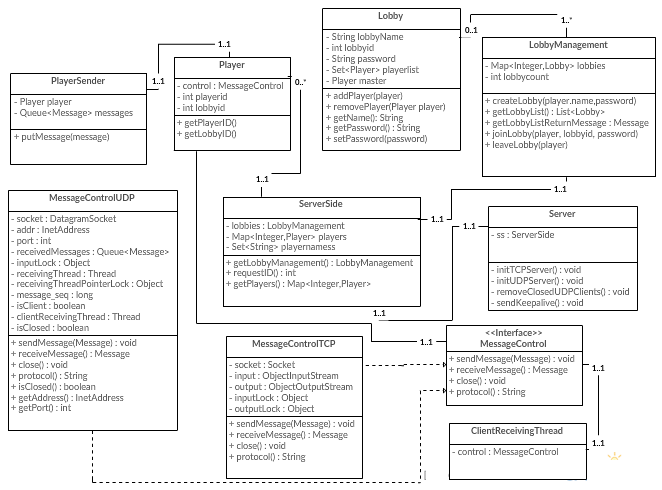
\includegraphics[width=600px,height=\textheight,keepaspectratio]{network_class_diagram}
\end{center}
\end{landscape}
%\end{landscape}}
\subsection{User Interface Class Diagram}
We have also created a class diagram to illustrate the classes of our user interface components.\\
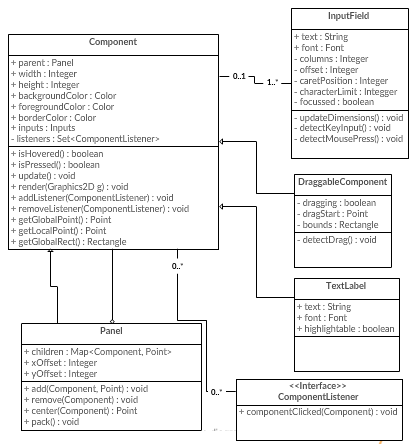
\includegraphics{user_interface_class_diagram}
\section{Software Architecture}
We have created a component diagram to model the static implementation view of the system, and to illustrate how components should communicate with other components in the system.\\
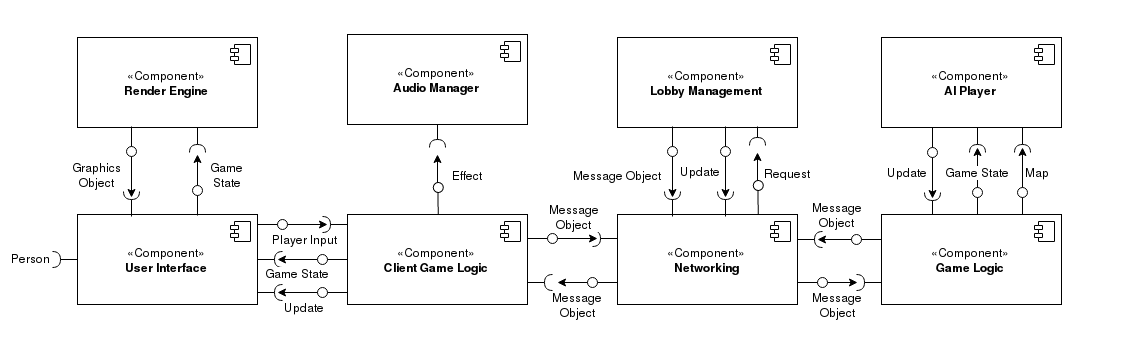
\includegraphics[width=550px,height=\textheight,keepaspectratio]{component_diagram}
\end{document}
